\clearpage
\section{Simulation model and method}
As seen in the previous section, initially there is a Gaussian wavepacket (see \refEq{eq: initial}) centered at $x_0$. To solve \refEq{eq: SG} efficiently, we constrain the boundary of the system to the left and right such that $-15\leq x\leq 15$. Within these boundaries, the position can be discretized according to

\iffalse
\begin{equation}
    x= \left(-\Delta \left({L-1\over 2}\right), -\Delta \left({L-1\over 2} -1\right)\right), \quad \text{with} \quad L=1201. 
\end{equation}
\fi

\begin{equation}
	x_i = -\Delta \left({L-1\over 2}-i\right), \quad \text{with} \quad i = 0,1,2,... , L-1.
\end{equation}
In that case, we have $L$ discrete grid points and the spatial resolution is given by $\Delta$.
In \T{python}, we implement this discretization of position using
\[
\texttt{x = np.linspace(-15,15,L)}.\footnote{this gives us an array with each point that we have discretized in position}
\]
With this discretization, the total wave function at any time $t$ is given by 
\begin{equation}
    \Phi(t) = \left(\begin{array}{c}
          \Phi_0(t)  \\
          \Phi_1(t)  \\
          \vdots  \\
          \Phi_{L-1}(t)
    \end{array}
    \right),
    \label{eq: discretPhi}
\end{equation}
where $\Phi_i (t)$ is the value of the wave function at position $x_i$ and time $t$.
Regarding the implementation into \T{python}, we use the function for the initial state \refEq{eq: initial} and calculate all the values for the positions defined in \texttt{x}. By doing so, we are left with an array of length $L$ containing the values of the wavefunctions. 
In addition to the discretization of $x$, the time is also discretized according to
\begin{equation}
    t = n\cdot \tau
\end{equation}
with $n$ ranging from $0$ to $m$. The idea of the algorithm is to update this array in small time steps such that we don't have to store the wavefunction at all times individually\footnote{Saving the wave function at each time step results in an enormous runtime and use of computing resources.}.


With the discretization of space, for the right-hand-side (RHS) of \refEq{eq: SG} it follows
 \begin{align}
    {\partial^2 \over \partial x^2}  \Phi(x,t)  &\longrightarrow \frac{\Phi(x_i+\Delta,t) - 2 \Phi(x_i,t) + \Phi(x_i-\Delta,t)}{\Delta^2}\\
        \intertext{and}
      V(x)  \Phi(x,t)  &\longrightarrow V(x_i) \Phi(x_i,t) \quad \text{with} \quad V(x) = {\Omega ^2 \over 2} x^2.
\end{align}
\clearpage
\noindent Employing the discretizations into the RHS of the Schr\"odinger equation and using \refEq{eq: discretPhi}, the differential equation can be written in matrix notation as
\begin{figure}[h!]
    \centering
    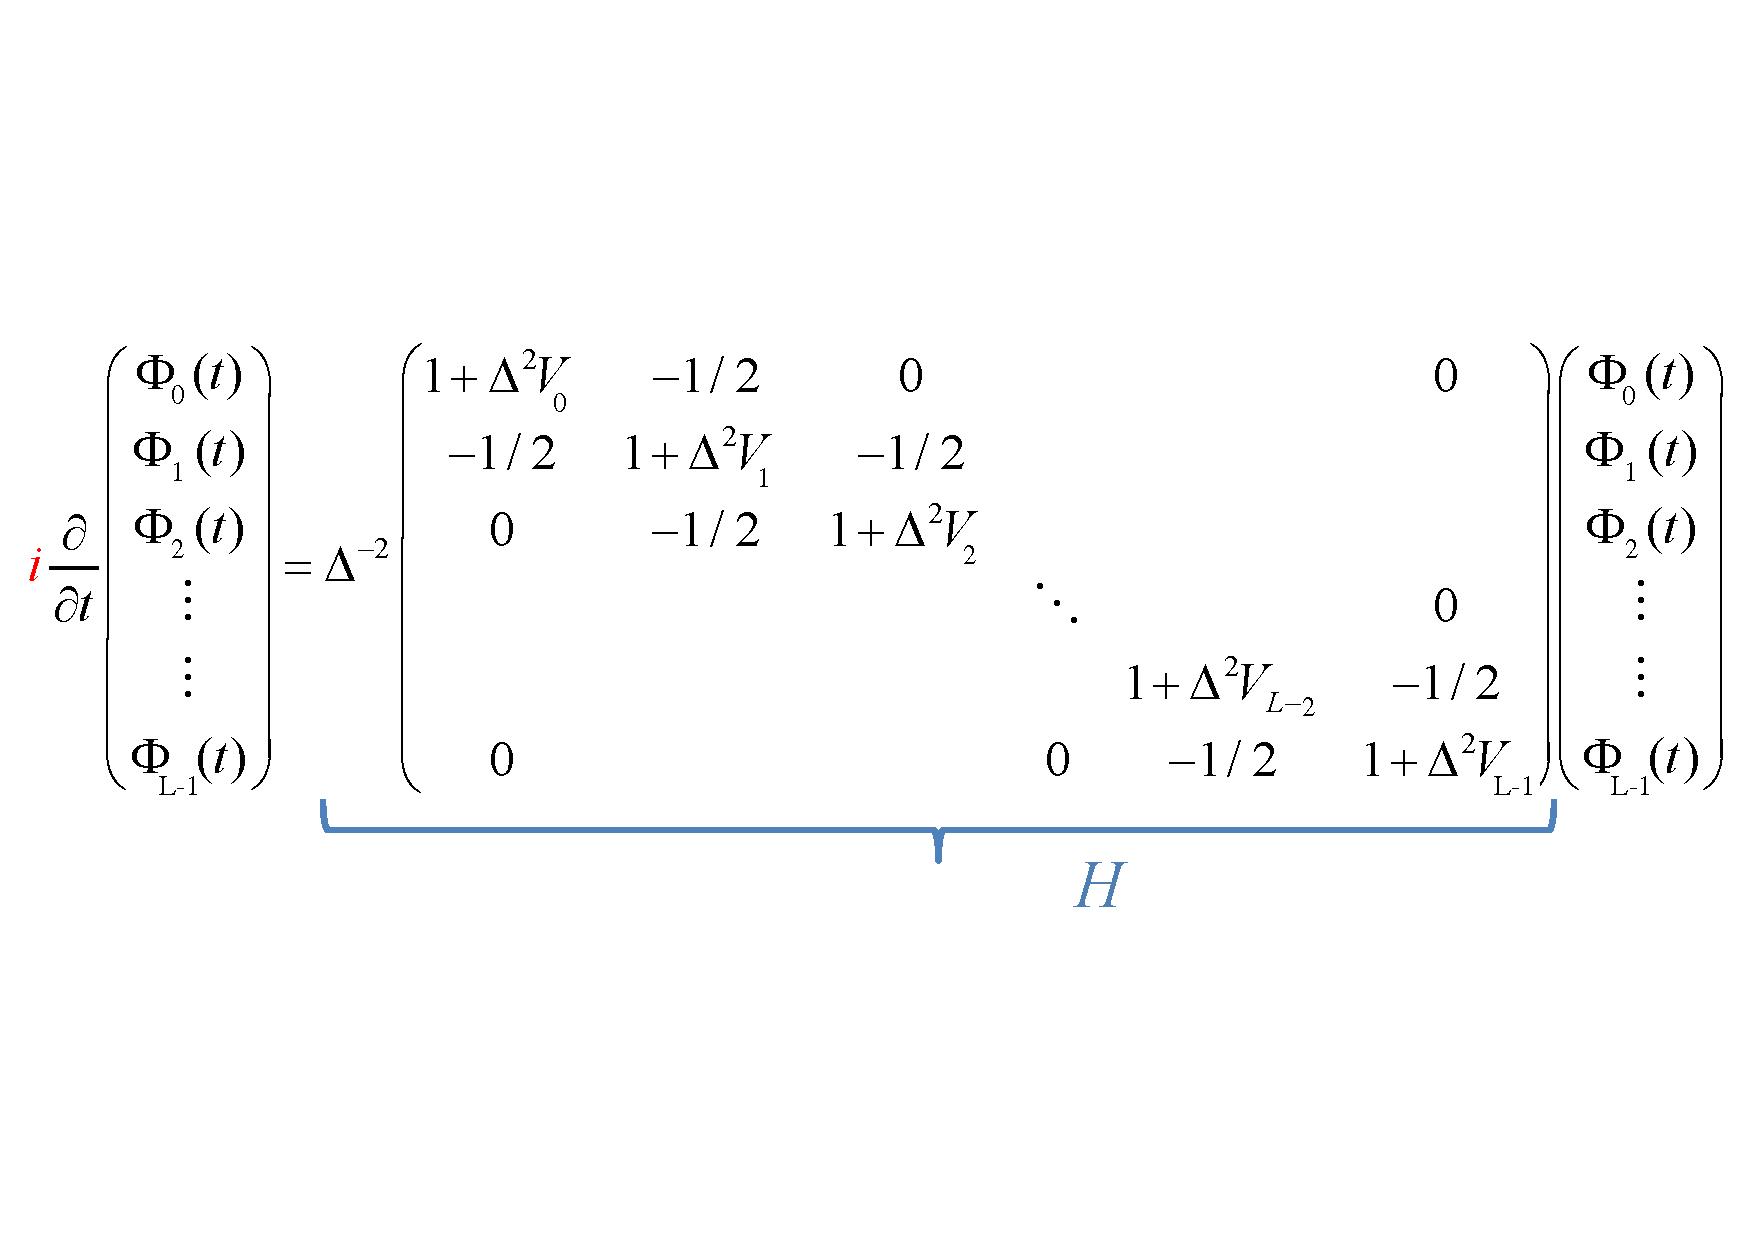
\includegraphics[width=.8 \textwidth]{Images/p39new.pdf}
\caption*{\tiny{source: Computational Physics - Lecture 17:
Time-dependent Schr\"odinger equation I (page 39)(edited)}}
\end{figure}

\noindent with $\Phi_i(t) = \Phi(x_i, t)$ and $V_i = V(x_i)$.

\noindent
The general solution for the Schr\"odinger equation is given by
\begin{equation}
    \Phi (x,t) = e^{-it\textcolor{NavyBlue}{H}}\Phi(x,t=0).
    \label{eq: gensol}
\end{equation}
Taking the exponential of $\textcolor{NavyBlue}{H}$ is cumbersome, which is why we resort to the use of second-order product formula approximation
\begin{equation}
     e^{-it \textcolor{NavyBlue}{H}}\approx \left(e^{-i\tau{K_1 \over 2}}e^{-i\tau{K_2 \over 2}} e^{-i\tau V}e^{-i\tau{K_2 \over 2}}e^{-i\tau{K_1 \over 2}}\right)^n = \left(e^{-i\tau \textcolor{NavyBlue}{H}}\right)^n.
     \label{eq: 2nd order}
\end{equation}
Our new task is to decompose $\textcolor{NavyBlue}{H}$, such that undertaking matrix exponentials is much easier. For that we decompose $\textcolor{NavyBlue}{H}$ into three different matrices $V,K_1,K_2$, such that
\begin{figure}[h!]
    \centering
    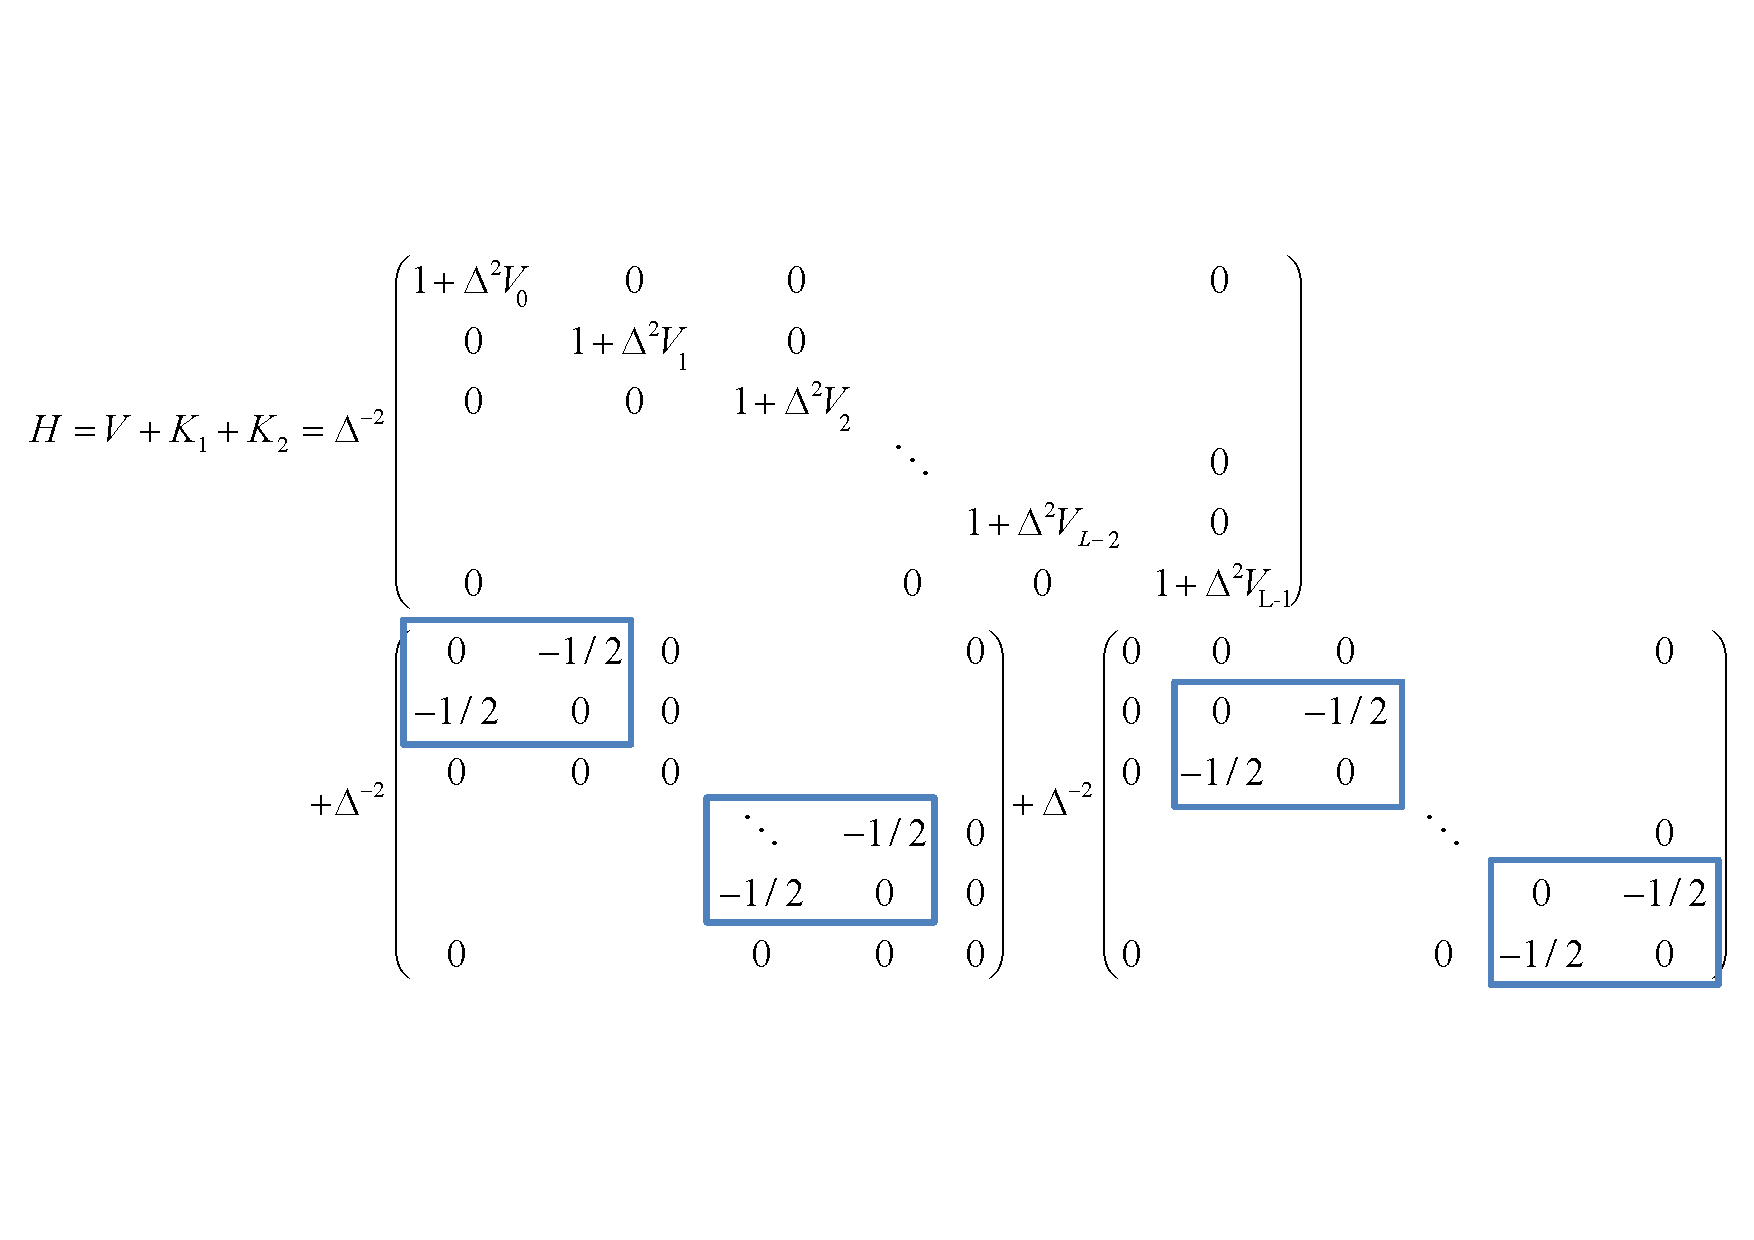
\includegraphics[width=.95 \textwidth]{Images/p49new.pdf}
\caption*{\tiny{source: Computational Physics - Lecture 17:
Time-dependent Schr\"odinger equation I (page 49)(edited)}}
\end{figure}
\clearpage
With the chosen decomposition, we see that the computation of $e^{-i\tau V}$ is very easy. It is a diagonal matrix with elements that are the exponentials of the diagonal elements. This is why calculating\footnote{$\Psi$ is an arbitrary array with the same dimensions as $\Phi$} 
\begin{align}
e^{-i\tau V}\Psi(x,t) &= \text{diag}(e^{-i\tau V_{00}},e^{-i\tau V_{11}},e^{-i\tau V_{22}},...,e^{-i\tau V_{(L-1)(L-1)}})\Psi(x,t)
\intertext{is done by }
e^{-i\tau V_{ii}}\Psi_i (t)&=\exp\left(-i\tau \underbrace{{1 \over \Delta ^2}(1+\Delta^2 V(x_i))}_{V_{ii}}\right)\Psi_i(t),
\label{eq: fynn}
\end{align}
with $i$ ranging from 0 to $L-1$. This corresponds to an elementwise multiplication of two arrays, which is implemented into \T{python} by creating an array consisting $\exp\left(-i \tau V_{ii}\right)$ at all positions $x_i$ and multiplying this with our array for $\Psi_i(t)$.\\

\noindent
For 
\begin{equation}
    e^{-i\frac{\tau}{2}{K_{1/2}}} \Psi(x,t),
\end{equation}
a different approach is chosen, due to the more complicated form of $K_{1/2}$.\footnote{$K_{1/2}$, which means either $K_1$ or $K_2$. } 
Fortunately, both $K_1$ and $K_2$ are composed of 2x2 matrices along the diagonal. Additionally, for $K_1$ the last entry is equal to zero, and for $K_2$, the first entry. To this end to multiply the matrices with $\Psi (x,t)$, we have to differentiate between the two cases
\begin{equation} 
\begin{split}
    &\exp \left(+ i{\tau\over 4\Delta^2 }
    \begin{pmatrix}
       0&1\\
       1&0\\
    \end{pmatrix}\right)
    \left(\begin{array}{c}
          \Phi _{k}(t)  \\
          \Phi _{k+1}(t)  \\
    \end{array}
    \right)\\ 
\end{split}
\end{equation}
and 
\begin{equation} \exp \left(+ i{\tau\over 4\Delta^2 }\cdot 0\right)
          \Phi(k,t) = \Phi(k,t).
          \label{eq: short}
\end{equation} 
It is easy to show that \refEq{eq: long} can be rewritten into
\begin{equation} 
    \exp \left(+ i{\tau\over 4\Delta^2 }
    \begin{pmatrix}
       0&1\\
       1&0\\
    \end{pmatrix}\right)
    \left(\begin{array}{c}
          \Phi _k (t)  \\
          \Phi _{k+1}(t)  \\
    \end{array}
    \right)
={\begin{pmatrix}
       \cos(a)&i \sin(a)\\
       i \sin(a)& \cos(a)\\
    \end{pmatrix}} \left(\begin{array}{c}
          \Phi _{k}(t)  \\
          \Phi _{k+1}(t)  \\
    \end{array}
    \right),
    \label{eq: long}
\end{equation}
with $a = {\tau\over 4\Delta^2 }$. With the last entry of $K_1$ being the zero entry, $k$ in \refEq{eq: long} must take all even numbers from $0$ to $L-2$. For $K_2$, the opposite is true, such that we have to take all the odd numbers from $1$ to $L-1$.\footnote{here, with $K_{1/2}$ we are referring to $e^{-i\tau{K_{1/2} \over 2}}$}$^,$\footnote{There is no need for an explicit implementation of \refEq{eq: short}, as doing no operation on an entry is the same as multiplying it by 1.}
The multiplication of a matrix with a vector is realized in \T{python} using \texttt{np.dot(a,b)}, which outputs the product of \T{a} and \T{b}. 
\clearpage
The index $k$ does not take all the numbers, but only the even ones for $K_1$ and the odd ones for $K_2$. To this end, choosing \texttt{for k in range(0,L-1,2)}, the counter \texttt{k} gets incremented by 2 in each step, such that with $k$ we have the even numbers and with $k+1$ the odd.

 In the code snippet below, we show the implementation of the function \T{dt(phi)}.
 Said function takes in a $\Phi (x,t)$ as an input and returns $\Phi (x,t+\tau)$, which is the wavefunction's evolution for one time step $\tau$. Calling this $n$ times iteratively, with the new input being the last output, results in the wavefunction at $t = n\tau$.\footnote{if the initial input was the $\Phi ({x,0})$}

\begin{lstlisting}[language=Python]
M    = np.array([[np.cos(a), 1j*np.sin(a)], [1j*np.sin(a), np.cos(a)]], dtype=np.complex128)  

def dt(phi):
    for k in range(0,len(phi)-1,2):             #K1
        phi[k:k+2] = np.dot(M,phi[k:k+2])
    for k in range(0,len(phi)-1,2):             #K2
        phi[k+1:k+3] = np.dot(M,phi[k+1:k+3])
    phi = Vx*phi                                #V part
    for k in range(0,len(phi)-1,2):             #K2
        phi[k+1:k+3] = np.dot(M,phi[k+1:k+3])
    for k in range(0,len(phi)-1,2):             #K1
        phi[k:k+2] = np.dot(M,phi[k:k+2])
    return phi
\end{lstlisting}

Using \T{phi[k:k+2]} (line 5 and 12 in code snippet), the vector $(\Phi_k,\Phi_{k+1})$ is sliced from the total array.\footnote{similar for the odd case (line 7 and 10 in code snippet)}\\

\noindent Apart from the wave function, we are interested in the probability density, defined as
\begin{equation}
P(x,t) = |\Phi(x,t)|^2 \quad \Rightarrow \quad  P(x_i,t) = |\Phi _i(t)|^2.\footnote{The absolute value can be calculated using \texttt{np.absolute()}.} \label{eq: P}	
\end{equation}


\noindent 
Next, we dedicate ourselves to the calculation of the mean position $\braket{x}$. According to \refEq{eq: scalar}, this is done by
\begin{align}
	\braket{x(t)} &= \Int{x|\Phi {(x,t)}|^2}.
\intertext{Due to the positions being discretized, we have }
x \rightarrow x_i, \qquad &|\Phi {(x,t)}|^2 \rightarrow |\Phi _i (t)|^2, \qquad dx \rightarrow \Delta \nonumber\\ 
\intertext{such that}
\braket{x_i(t)}&= \sum _{i = 0}^{L-1} x_i P(x_i,t) \Delta.\label{eq: x dis}
\intertext{Similarly, for $\braket{x^2}$ we have}
\braket{x_i^2(t)}&= \sum _{i = 0}^{L-1} x_i^2 P(x_i,t) \Delta.\label{eq: xx dis}
\end{align}
These two sums (\refEq{eq: x dis} and \refEq{eq: xx dis}), can be implemented into \T{python} using
\[
\braket{x_i(t)} = \T{np.sum(x*P*Delta)} \qquad \text{and} \qquad  \braket{x_i^2(t)} = \T{np.sum(x**2*P*Delta)},
\]
with $\T{P} = P(x_i,t)$. From there the variance can be calculated according to \refEq{eq: var} from \refEq{eq: x dis} and \refEq{eq: xx dis}:
\[
\text{Var}(x_i) = \braket{x_i^2(t)} - \braket{x_i(t)}^2.
\]